\begin{enumerate}[label=\thechapter.\arabic*,ref=\thechapter.\theenumi]
\item For the ordinary differential equation
\begin{align*}
\frac{d^3y}{dt^3} + 6\frac{d^2y}{dt^2} + 11\frac{dy}{dt} + 6y = 1,
\end{align*}
with initial conditions $y(0) = y'(0) = y''(0) = y'''(0) = 0$, the value of 
\begin{align*}
\lim_{{t \to \infty}} y(t) &= ?
\end{align*}
(round off to $3$ decimal places).
\hfill(GATE CH 2021)\\
\solution
\iffalse
\documentclass[journal,12pt,twocolumn]{IEEEtran}
\usepackage{cite}
\usepackage{amsmath,amssymb,amsfonts,amsthm}
\usepackage{algorithmic}
\usepackage{graphicx}
\usepackage{textcomp}
\usepackage{xcolor}
\usepackage{listings}
\usepackage{enumitem}
\usepackage{mathtools}
\usepackage{gensymb}
\usepackage{comment}
\usepackage[breaklinks=true]{hyperref}
\usepackage{tkz-euclide}
\usepackage{gvv} 
\def\inputGnumericTable{} 
\usepackage[latin1]{inputenc} 
\usepackage{color} 

\newtheorem{theorem}{Theorem}[section]
\newtheorem{problem}{Problem}
\newtheorem{proposition}{Proposition}[section]
\newtheorem{lemma}{Lemma}[section]
\newtheorem{corollary}[theorem]{Corollary}
\newtheorem{example}{Example}[section]
\newtheorem{definition}[problem]{Definition}
\newcommand{\BEQA}{\begin{eqnarray}}
\newcommand{\EEQA}{\end{eqnarray}}
\newcommand{\define}{\stackrel{\triangle}{=}}
\theoremstyle{remark}
\newtheorem{rem}{Remark}

\begin{document}

\bibliographystyle{IEEEtran}
\vspace{3cm}

\title{GATE 2022-IN}
\author{EE23BTECH1205 - Avani Chouhan$^{*}$}
\maketitle
\newpage
\bigskip

\renewcommand{\thefigure}{\theenumi}
\renewcommand{\thetable}{\theenumi}

\vspace{3cm}
\textbf{Question : 18} \\
A signal \( x(t) \) is band-limited between 100 Hz and 200 Hz. A signal \( y(t) \) is related to \( x(t) \) as follows:\\

\( y(t) = x(2t - 5) \)\\
The statement that is always true is \\

\begin{enumerate}
  \item[(A)] \( y(t) \) is band-limited between 50 Hz and 100 Hz
  \item[(B)] \( y(t) \) is band-limited between 100 Hz and 200 Hz
  \item[(C)] \( y(t) \) is band-limited between 200 Hz and 400 Hz
  \item[(D)] \( y(t) \) is not band-limited 
\end{enumerate}

\hfill{(GATE IN 2022)}\\
\textbf{Solution:} \\
\fi
\begin{align}
x(t) &\rightleftharpoons X(\omega) \label{eq1}\\
x(at) &\rightleftharpoons \frac{1}{|a|} X\left(\frac{\omega}{a}\right) \label{eq2}\\
x(2t) &\rightleftharpoons \frac{1}{2} X\left(\frac{\omega}{2}\right) \label{eq3}\\
x(t - t_0) &\rightleftharpoons e^{-j\omega t_0}X(\omega) \label{eq4}\\
x(2t - 5) &\rightleftharpoons e^{-j5\omega} \cdot \frac{1}{2} X\left(\frac{\omega}{2}\right) \label{eq5}
\end{align}

The operation \(x(2t-5)\) compresses time by a factor of 2 and shifts 5 units rightward. This expands the frequency domain, doubling the bandwidth of \(x(t)\) from 100 Hz to 200 Hz to \(y(t)\) between 200 Hz and 400 Hz.\\

Hence, the correct answer is option (C).

%\end{document}


\pagebreak
\item \textbf{Question:}
Consider the differential equation \\$\frac{d^2y}{dx^2}+8\frac{dy}{dx}+16y=0$ and the boundary conditions $y(0)=1$ and $\frac{dy}{dx}(0)=0$. The solution to equation is:\\
\hfill{(GATE.AE-1.2021)}\\
\solution
 \iffalse
\let\negmedspace\undefined
\let\negthickspace\undefined
\documentclass[journal,12pt,twocolumn]{IEEEtran}
\usepackage{xparse}
\usepackage{cite}
\usepackage{amsmath,amssymb,amsfonts,amsthm}
\usepackage{algorithmic}
\usepackage{graphicx}
\usepackage{textcomp}
\usepackage{xcolor}
\usepackage{txfonts}
\usepackage{listings}
\usepackage{enumitem}
\usepackage{mathtools}
\usepackage{gensymb}
\usepackage{comment}
\usepackage[breaklinks=true]{hyperref}
\usepackage{tkz-euclide}
\usepackage{listings}
\usepackage{gvv}
\def\inputGnumericTable{}
\usepackage[latin1]{inputenc}
\usepackage{color}
\usepackage{array}
\usepackage{longtable}
\usepackage{calc}
\usepackage{multirow}
\usepackage{hhline}
\usepackage{ifthen}
\usepackage{lscape}
\begin{enumerate}[label=\thechapter.\arabic*,ref=\thechapter.\theenumi]
\numberwithin{equation}{enumi}
\numberwithin{figure}{enumi}
\numberwithin{table}{enumi}
\item Laplace Transform of Partial Differentials\\
Let a function $y\brak{x,t}$ be defined for all $t>0$ and assumed to be bounded. Appling Laplace transform in t considering x as a parameter,
\begin{align}
 \mathcal{L}\brak{y\brak{x,t}} &= \int_{0}^{\infty}e^{-st}y\brak{x,t}dt\\
 &= Y\brak{x,s}
\end{align}
Let $\dfrac{\partial y\brak{x,t}}{\partial t}$ be $y_t\brak{x,t}$ and $\dfrac{\partial y\brak{x,t}}{\partial x}$ be $y_x\brak{x,t}$, then
\begin{align}
 \mathcal{L}\brak{y_t\brak{x,t}} &= \int_{0}^{\infty}e^{-st}y_t\brak{x,t}dt\\
 &= \left. e^{-st}y\brak{x,t}\right|_{0}^{\infty} + s\int_{0}^{\infty}e^{-st} y\brak{x,t} dt\\
 &= sY\brak{x,s} - y\brak{x,0} \label{L(y_t(x,t))}\\
 \mathcal{L}\brak{y_x\brak{x,t}} &= \int_{0}^{\infty}e^{-st}y_x\brak{x,t}dt\\
 &= \dfrac{d}{dx}\int_{0}^{\infty}e^{-st}y\brak{x,t}dt \label{L(y_x(x,t))}\\
 &= \dfrac{dY\brak{x,s}}{dx}
\end{align}
\item Laplace transform of f(t):
\begin{align}
        f(t)u(t)\system{L}&\int_{0}^{\infty}f(t)e^{-st}\; dt\\
        &=F(s)\label{lap transform}
\end{align}
\item Laplace transform of powers of $t$\\
        Let $f(t)=t^nu(t)$\\
From \eqref{lap transform},and considering $h=st$
\begin{align}
        F(s)&=\frac{1}{s^{n+1}}\int_{0}^{\infty}h^ne^{-h}\;dh\label{lap 1}\\
        (n-1)!&=\int_0^\infty e^{-t}t^{n-1}\;dt\text{ (Gamma function)}\label{gamma}
\end{align}
From \eqref{lap 1},\eqref{gamma}
\begin{align}
        F(s)&=\frac{n!}{s^{n+1}}\\
         t^nu(t)&\system{L}\frac{n!}{s^{n+1}}\label{lap exp}
\end{align}
\item Frequency shift property:\\
        Let $f(t)=y(t)e^{-at}u(t)$\\
From\eqref{lap transform},
\begin{align}
        F(s)&=\int_0^{\infty}y(t)e^{-(s+a)t}\;dt\\
         y(t)e^{-at}u(t)&\system{L}Y(s+a)\label{lap freq shift}
\end{align}
\item Inverse Laplace for partial fractions\\
From \eqref{lap exp},\eqref{lap freq shift} we get
\begin{align}
    &\frac{b}{(s+a)^n}\xleftrightarrow{\mathcal{L}^{-1}}\frac{b}{(n-1)!}\cdot t^{n-1} e^{-at}\cdot u(t)\label{inv lap (partial fractions)}
\end{align}
\item Laplace transform of derivatives:\\
        Let $f(t)=y'(t)u(t)$\\
From \eqref{lap transform}, integration by parts,recursion
\begin{align}
        F(s)&=\int_{0}^\infty e^{-st}\; dy\\
        &=[y(t)e^{-st}]_0^\infty+s\int_0^\infty y(t)e^{-st}dt\\
        &=-y(0)+sY(s)\label{lap 2}
\end{align}
From\eqref{lap 2},recursion
\begin{align}
        y'(t)u(t)&\system{L}sY(s)-\int y'(t)\;dt\vert_{t=0}\\
        y^{(n)}(t)u(t)&\system{L}s^nY(s)-\sum\limits_{k=0}^{n-1}s^{(n-1-k)}y^{(k)}(0)\label{lap (derivatives)}
\end{align}
\end{enumerate}

\newtheorem{theorem}{Theorem}[section]
\newtheorem{problem}{Problem}
\newtheorem{proposition}{Proposition}[section]
\newtheorem{lemma}{Lemma}[section]
\newtheorem{corollary}[theorem]{Corollary}
\newtheorem{example}{Example}[section]
\newtheorem{definition}[problem]{Definition}
\newcommand{\BEQA}{\begin{eqnarray}}
\newcommand{\EEQA}{\end{eqnarray}}
\newcommand{\define}{\stackrel{\triangle}{=}}
\theoremstyle{remark}
\newtheorem{rem}{Remark}
\begin{document}

\bibliographystyle{IEEEtran}
\vspace{3cm}

\title{GATE-AE.1}
\author{EE23BTECH11046 - Poluri Hemanth$^{*}$}
\maketitle
\textbf{Question:}
Consider the differential equation \\$\frac{d^2y}{dx^2}+8\frac{dy}{dx}+16y=0$ and the boundary conditions $y(0)=1$ and $\frac{dy}{dx}(0)=0$. The solution to equation is:\\
\hfill{(GATE.AE-1.2021)}\\
\textbf{Solution:}\\
\fi
\begin{table}[h!]
    % Change address in github
        \begin{table}[ht!]
\centering
\begin{tabular}{ |c|c|c| } 
 \hline
Symbols & Description & Values  \\
\hline
 $V_s$ & Input voltage & 220 V and 50Hz\\
 \hline
 $\chi_L$ & Impedance across inductor & $j\omega L$\\
 \hline
 $\chi_C$ & Impedance across capacitor & $\frac{-j}{\omega C}$\\
 \hline
 $Z$& Impedance across the entire circuit & $\frac{1}{R+j\omega L +\frac{-j}{\omega C}}$\\
 \hline
\end{tabular}
\caption{Parameters, Descriptions, and Values}
\label{table:ee25-bm54-gate2022}
\end{table}




        \caption{Parameters}
\end{table}\\
From \ref{lap (derivatives)}
\begin{align}
	\frac{d^2y}{dx^2}+8\frac{dy}{dx}+16y&\Large\xleftrightarrow{\mathcal{L}}s^2Y(s)-sy(0)-y'(0)+8sY(s)-8y(0)+16Y(s)
\end{align}
\begin{align}
	Y(s)(s^2+8s+16)&=s+8
\end{align}
\begin{align}
	\Rightarrow Y(s)&=\frac{s+8}{s^2+8s+16}\\
	&=\frac{1}{s+4}+\frac{4}{(s+4)^2}\label{1ae.1}
\end{align}
For inversion of $Y(s)$ in partial fractions-
\\ From \ref{inv lap (partial fractions)}
\begin{align}
	&\frac{b}{(s+a)^n}\Large\xleftrightarrow{\mathcal{L}^{-1}}\frac{b}{(n-1)!}\cdot x^{n-1} e^{-ax}\cdot u(x)\label{invae.1}
\end{align}
\\
Applying Laplace inverse-\\
\\From \eqref{1ae.1},\eqref{invae.1}
\begin{align}
	y(x)&=\frac{1}{0!} e^{-4x}\cdot u(x)+\frac{4}{1!}x\cdot e^{-4x}\cdot u(x)\\
	&=(1+4x)e^{-4x}u(x)
\end{align}
\newpage
\begin{figure}[h!]
    \centering
    \includegraphics[width=1\linewidth]{2021/AE/1/figures/figure.png}
        \caption{Plot of y(x)}
\end{figure}


%\end{document}






\pagebreak
\item\textbf{Question:}
The solution of second-order differential equation \\ $\frac{d^2y}{dx^2}+2\frac{dy}{dx}+y=0$ with boundary conditions $y(0)=1$ and $y(1)=3$.\\
\hfill{(GATE  2021 CE.26)}\\
\solution
\iffalse
\let\negmedspace\undefined
\let\negthickspace\undefined
\documentclass[journal,12pt,twocolumn]{IEEEtran}
\usepackage{xparse}
\usepackage{cite}
\usepackage{amsmath,amssymb,amsfonts,amsthm}
\usepackage{algorithmic}
\usepackage{graphicx}
\usepackage{textcomp}
\usepackage{xcolor}
\usepackage{txfonts}
\usepackage{listings}
\usepackage{enumitem}
\usepackage{mathtools}
\usepackage{gensymb}
\usepackage{comment}
\usepackage[breaklinks=true]{hyperref}
\usepackage{tkz-euclide}
\usepackage{listings}
\usepackage{gvv}
\def\inputGnumericTable{}
\usepackage[latin1]{inputenc}
\usepackage{color}
\usepackage{array}
\usepackage{longtable}
\usepackage{calc}
\usepackage{multirow}
\usepackage{hhline}
\usepackage{ifthen}
\usepackage{lscape}
\begin{enumerate}[label=\thechapter.\arabic*,ref=\thechapter.\theenumi]
\numberwithin{equation}{enumi}
\numberwithin{figure}{enumi}
\numberwithin{table}{enumi}
\item Laplace Transform of Partial Differentials\\
Let a function $y\brak{x,t}$ be defined for all $t>0$ and assumed to be bounded. Appling Laplace transform in t considering x as a parameter,
\begin{align}
 \mathcal{L}\brak{y\brak{x,t}} &= \int_{0}^{\infty}e^{-st}y\brak{x,t}dt\\
 &= Y\brak{x,s}
\end{align}
Let $\dfrac{\partial y\brak{x,t}}{\partial t}$ be $y_t\brak{x,t}$ and $\dfrac{\partial y\brak{x,t}}{\partial x}$ be $y_x\brak{x,t}$, then
\begin{align}
 \mathcal{L}\brak{y_t\brak{x,t}} &= \int_{0}^{\infty}e^{-st}y_t\brak{x,t}dt\\
 &= \left. e^{-st}y\brak{x,t}\right|_{0}^{\infty} + s\int_{0}^{\infty}e^{-st} y\brak{x,t} dt\\
 &= sY\brak{x,s} - y\brak{x,0} \label{L(y_t(x,t))}\\
 \mathcal{L}\brak{y_x\brak{x,t}} &= \int_{0}^{\infty}e^{-st}y_x\brak{x,t}dt\\
 &= \dfrac{d}{dx}\int_{0}^{\infty}e^{-st}y\brak{x,t}dt \label{L(y_x(x,t))}\\
 &= \dfrac{dY\brak{x,s}}{dx}
\end{align}
\item Laplace transform of f(t):
\begin{align}
        f(t)u(t)\system{L}&\int_{0}^{\infty}f(t)e^{-st}\; dt\\
        &=F(s)\label{lap transform}
\end{align}
\item Laplace transform of powers of $t$\\
        Let $f(t)=t^nu(t)$\\
From \eqref{lap transform},and considering $h=st$
\begin{align}
        F(s)&=\frac{1}{s^{n+1}}\int_{0}^{\infty}h^ne^{-h}\;dh\label{lap 1}\\
        (n-1)!&=\int_0^\infty e^{-t}t^{n-1}\;dt\text{ (Gamma function)}\label{gamma}
\end{align}
From \eqref{lap 1},\eqref{gamma}
\begin{align}
        F(s)&=\frac{n!}{s^{n+1}}\\
         t^nu(t)&\system{L}\frac{n!}{s^{n+1}}\label{lap exp}
\end{align}
\item Frequency shift property:\\
        Let $f(t)=y(t)e^{-at}u(t)$\\
From\eqref{lap transform},
\begin{align}
        F(s)&=\int_0^{\infty}y(t)e^{-(s+a)t}\;dt\\
         y(t)e^{-at}u(t)&\system{L}Y(s+a)\label{lap freq shift}
\end{align}
\item Inverse Laplace for partial fractions\\
From \eqref{lap exp},\eqref{lap freq shift} we get
\begin{align}
    &\frac{b}{(s+a)^n}\xleftrightarrow{\mathcal{L}^{-1}}\frac{b}{(n-1)!}\cdot t^{n-1} e^{-at}\cdot u(t)\label{inv lap (partial fractions)}
\end{align}
\item Laplace transform of derivatives:\\
        Let $f(t)=y'(t)u(t)$\\
From \eqref{lap transform}, integration by parts,recursion
\begin{align}
        F(s)&=\int_{0}^\infty e^{-st}\; dy\\
        &=[y(t)e^{-st}]_0^\infty+s\int_0^\infty y(t)e^{-st}dt\\
        &=-y(0)+sY(s)\label{lap 2}
\end{align}
From\eqref{lap 2},recursion
\begin{align}
        y'(t)u(t)&\system{L}sY(s)-\int y'(t)\;dt\vert_{t=0}\\
        y^{(n)}(t)u(t)&\system{L}s^nY(s)-\sum\limits_{k=0}^{n-1}s^{(n-1-k)}y^{(k)}(0)\label{lap (derivatives)}
\end{align}
\end{enumerate}

\newtheorem{theorem}{Theorem}[section]
\newtheorem{problem}{Problem}
\newtheorem{proposition}{Proposition}[section]
\newtheorem{lemma}{Lemma}[section]
\newtheorem{corollary}[theorem]{Corollary}
\newtheorem{example}{Example}[section]
\newtheorem{definition}[problem]{Definition}
\newcommand{\BEQA}{\begin{eqnarray}}
\newcommand{\EEQA}{\end{eqnarray}}
\newcommand{\define}{\stackrel{\triangle}{=}}
\theoremstyle{remark}
\newtheorem{rem}{Remark}
\begin{document}

\bibliographystyle{IEEEtran}
\vspace{3cm}

\title{GATE-CE.26}
\author{EE23BTECH11046 - Poluri Hemanth$^{*}$}
\maketitle
\textbf{Question:}
The solution of second-order differential equation \\ $\frac{d^2y}{dx^2}+2\frac{dy}{dx}+y=0$ with boundary conditions $y(0)=1$ and $y(1)=3$.\\
\hfill{(GATE  2021 CE.26)}\\
\textbf{Solution:}
\fi
\begin{table}[h!]
    % Change address in github
        \begin{table}[ht!]
\centering
\begin{tabular}{ |c|c|c| } 
 \hline
Symbols & Description & Values  \\
\hline
$R$ & Residue Formula &$\frac{1}{\brak {m-1}!}\lim\limits_{s\to a}\frac{d^{m-1}}{ds^{m-1}}\brak {{(s-a)}^{m}f\brak se^{st}}$\\
 \hline
 $\phi(x)$ & Transformation of $y(x)$ & $y(x+1)$\\
 \hline
$g(x)$ & Euler's Approximated function of f(x) & $g_{(n-1)}(x) + hf'\brak{x_{n-1},y_{n-1}}$\\
 \hline
 $h$ & Step-size & $0.2$\\
 \hline
\end{tabular}
\caption{Parameters, Descriptions, and Values}
\label{table:ee25-ce48-gate2022}
\end{table}




        \caption{Parameters}
        \label{tab:es.47}
\end{table}\\
Applying Laplace transform
\\From \ref{lap (derivatives)}
\begin{align}
	\frac{d^2y}{dx^2}+2\frac{dy}{dx}+y&\Large\xleftrightarrow{\mathcal{L}}s^2Y(s)-sy(0)-y'(0)+2sY(s)-2y(0)+Y(s)
\end{align}
\begin{align}
	Y(s)(s^2+2s+1)&=s-2-y'(0)
\end{align}
\begin{align}
	\Rightarrow Y(s)&=\frac{s-2-y'(0)}{s^2+2s+1}\\
	&=\frac{1}{s+1}-\frac{2+y'(0)}{(s+1)^2}\label{1ce.1}
\end{align}
For inversion of $Y(s)$ in partial fractions-
\\From \ref{inv lap (partial fractions)}
\begin{align}
	&\frac{b}{(s+a)^n}\system{L}\frac{b}{(n-1)!}\cdot x^{n-1} e^{-ax}\cdot u(x)\label{invce.26}
\end{align}
Applying Laplace inverse-\\
\\From \eqref{1ce.1},\eqref{invce.26}
\begin{align}
	y(x)&=\frac{1}{0!} e^{-x}\cdot u(x)-\frac{3+y'(0)}{1!}x\cdot e^{-x}\cdot u(x)\\
	&=(1-(3+y'(0))x)e^{-x}u(x)\label{yce.26}
\end{align}
From \eqref{yce.26},
\begin{align}
	y(1)&=(1-3-y'(0))e^{-1}\\
	3&=(1-3-y'(0))e^{-1}\\
	\Rightarrow y'(0)&=-(2+3e)\label{y'0ce.26}
\end{align}
From\eqref{y'0ce.26},\eqref{yce.26}
\begin{align}
	y(x)=(e^x+(3e-1)xe^{-x})u(x)
\end{align}
\\
\\
\\
\\
\\
\\
\\
\\
\\
\\
\\
\\
\\
\\
\begin{figure}[h!]
    \centering
    \includegraphics[width=1\linewidth]{2021/CE/26/figures/figure1.png}
        \caption{Plot of y(x)}
    \label{fig:enter-label}
\end{figure}


%\end{document}





\pagebreak
\item A system has a transfer function
\begin{align}
    G(s) = \frac{3e^{-4s}}{12s + 1}\nonumber
\end{align}
When a step-change of magnitude $M$ is given to the system input, the final value of the system output is measured to be 120. The value of M is \_\_\_\_\_.
\hfill(GATE 2021 CH Q52)\\
\solution
\iffalse
\let\negmedspace\undefined
\let\negthickspace\undefined
\documentclass[journal,12pt,twocolumn]{IEEEtran}
\usepackage{cite}
\usepackage{amsmath,amssymb,amsfonts,amsthm}
\usepackage{algorithmic}
\usepackage{graphicx}
\usepackage{textcomp}
\usepackage{xcolor}
\usepackage{txfonts}
\usepackage{listings}
\usepackage{enumitem}
\usepackage{mathtools}
\usepackage{gensymb}
\usepackage{comment}
\usepackage[breaklinks=true]{hyperref}
\usepackage{tkz-euclide} 
\usepackage{listings}
\usepackage{gvv}                            \usepackage{tikz}
\usepackage{circuitikz}
\def\inputGnumericTable{}                                
\usepackage[latin1]{inputenc}                            
\usepackage{color}                                       
\usepackage{array}                                       
\usepackage{longtable}                                   
\usepackage{calc}                              
\usepackage{tikz}
\usepackage{multirow}                                    
\usepackage{hhline}                                      
\usepackage{ifthen}                            
\usepackage{caption}
\usepackage{lscape}
\usepackage{amsmath}
\newtheorem{theorem}{Theorem}[section]
\newtheorem{problem}{Problem}
\newtheorem{proposition}{Proposition}[section]
\newtheorem{lemma}{Lemma}[section]
\newtheorem{corollary}[theorem]{Corollary}
\newtheorem{example}{Example}[section]
\newtheorem{definition}[problem]{Definition}
\newcommand{\BEQA}{\begin{eqnarray}}
\newcommand{\EEQA}{\end{eqnarray}}
\newcommand{\define}{\stackrel{\triangle}{=}}
\theoremstyle{remark}
\newtheorem{rem}{Remark}

\begin{document}

\bibliographystyle{IEEEtran}
\vspace{3cm}

\title{GATE 2021 CH Q52}
\author{EE23BTECH11009 - AROSHISH PRADHAN$^{*}$% <-this % stops a space
}
\maketitle
\newpage
\bigskip
\textbf{Question:} A system has a transfer function
\begin{align}
    G(s) = \frac{3e^{-4s}}{12s + 1}\nonumber
\end{align}
When a step-change of magnitude $M$ is given to the system input, the final value of the system output is measured to be 120. The value of M is \_\_\_\_\_.
\hfill(GATE 2021 CH Q52)\\
\solution
\fi
\begin{table}[!h]
    \centering
    \begin{tabular}{|c|c|c|}
    \hline
       \textbf{Symbol}  & \textbf{Value} & \textbf{Description}\\
    \hline
        $x(t)$ & $Mu(t)$ & Input Signal\\
    \hline
        $X(s)$ & $\frac{M}{s}$ & s-domain Input Signal\\
    \hline
        $y(t)$ &  & Output Signal\\
    \hline
        $Y(s)$ & & s-domain Output Signal\\
    \hline
       $G(s)$ & $\frac{3e^{-4s}}{12s + 1}$ & Transfer Function\\
    \hline
    \end{tabular}
    \caption{Given Parameters}
    \label{tab:1_gate.21.ch.52}
\end{table}


Given, input step-change:
\begin{align}
    x(t) &= Mu(t)\\
    u(t) &\system{L} \frac{1}{s}\\
    \implies X(s) &= \frac{M}{s}
\end{align}
Transfer Function:
\begin{align}
    G(s) &= \frac{Y(s)}{X(s)} = \frac{3e^{-4s}}{12s + 1}\\
    \implies Y(s) &= \frac{3e^{-4s}}{12s + 1}\frac{M}{s}
\end{align}
$\therefore$ system output
\begin{align}
     \lim_{s\rightarrow0}sY(s) &= 120\\
    \implies \lim_{s\rightarrow0}\brak{\frac{3e^{-4s}}{12s + 1}M} &= 120\\
    \implies 3M &= 120\\
    \implies M &= 40
\end{align}

\begin{figure}
    \centering
    \includegraphics[width = \columnwidth]{2021/CH/52/figs/assign9.png}
	\caption{Plot of $G(s)$ vs $s$}
    \label{fig:1_gate.21.ch.52}
\end{figure}
%\end{document}

\pagebreak
\item The Bode magnitude plot for the transfer function $\frac{V_o(s)}{V_i(s)}$ of the circuit is as shown. The value of R is \_\_\_\_\_$\Omega$. \hfill(GATE 2021 EE Q20)
\begin{figure}[!ht]
    \centering
    \tikzset{
    block/.style = {draw, fill=white, rectangle, minimum height=3em, minimum width=3em},
    tmp/.style  = {coordinate}, 
    minus/.style= {draw, fill=white, circle, node distance=1cm, append after command={\pgfextra \draw ($(\tikzlastnode.center) + (-0.15,0)$) -- ($(\tikzlastnode.center) + (0.15,0)$) node[above] {$-$}; \endpgfextra}},
    plus/.style= {draw, fill=white, circle, node distance=1cm, append after command={\pgfextra \draw ($(\tikzlastnode.center) + (-0.15,0)$) -- ($(\tikzlastnode.center) + (0.15,0)$) node[above] {$+$}; \endpgfextra}},
    input/.style = {coordinate},
    output/.style= {coordinate},
    pinstyle/.style = {pin edge={to-,thin,black}}
}


\begin{tikzpicture}[auto, node distance=2cm]
    % Blocks
    \node [input, name=rinput] (rinput) at (0,0) {};
    \node [minus] (sum1) at (1,0) {};
    \node [block] (controller) at (3,0) {$K_{p}$};
    \node [block] (kd) at (3,-2) {$sK_D$};
    \node [block] (up) at (3,2) {\Large$\frac{K_{i}}{s}$};
    \node [plus] (sum2) at (5,0) {};
    \node [block] (system) at (7,0) {$P\brak{s}=\frac{1}{\brak{s+1}\brak{s+2}}$};
    \node [output] (output) at (9,0) {};
    \node [tmp] (tmp1) at (3,-4) {$H(s)$};

    % Connectors
    \draw [->] (rinput) -- node[below]{$r\brak{t}$} (sum1);
    \draw [->] (sum1) -- node[name=z,anchor=north,fill=white,circle,inner sep=1pt]{$e\brak{t}$} (controller);
    \draw [->] (controller) -- (sum2);
    \draw [->] (sum2) -- node[above, pos=-2.5]{$G_c\brak{t}$} (system);
    \draw [->] (system) -- node [pos = 1,name=y] {$L\brak{t}$} (output);
    \draw [->] (z) |- (up);
    \draw [->] (up) -| (sum2);
    \draw [->] (z) |- (kd);
    \draw [->] (kd) -| (sum2);
    \draw [->] (y) |- (tmp1);
    \draw [->] (tmp1) -| (sum1);
\end{tikzpicture}

\end{figure}
\begin{figure}[!ht]
    \centering
    \includegraphics[width=\columnwidth]{2021/EE/20/figs/bode.png}
\end{figure}
\solution
 \iffalse
\let\negmedspace\undefined
\let\negthickspace\undefined
\documentclass[journal,12pt,onecolumn]{IEEEtran}
\usepackage{cite}
\usepackage{amsmath,amssymb,amsfonts,amsthm}
\usepackage{algorithmic}
\usepackage{graphicx}
\usepackage{textcomp}
\usepackage{xcolor}
\usepackage{txfonts}
\usepackage{listings}
\usepackage{enumitem}
\usepackage{mathtools}
\usepackage{gensymb}
\usepackage{comment}
\usepackage[breaklinks=true]{hyperref}
\usepackage{tkz-euclide} 
\usepackage{tikz}
\usepackage{circuitikz}
%\usetikzlibrary{circuits.ee.IEC}
\usepackage{listings}
\usepackage{gvv} 
\usepackage{caption}
\def\inputGnumericTable{}                   

%\usepackage[latin1]{inputenc}                                
\usepackage{color}                                            
\usepackage{array}                                            
\usepackage{longtable}                                       
\usepackage{calc}                                             
\usepackage{multirow}                                         
\usepackage{hhline}                                           
\usepackage{ifthen}                                           
\usepackage{lscape}
\usepackage{tikz}
\usepackage{circuitikz}

\newtheorem{theorem}{Theorem}[section]
\newtheorem{problem}{Problem}
\newtheorem{proposition}{Proposition}[section]
\newtheorem{lemma}{Lemma}[section]
\newtheorem{corollary}[theorem]{Corollary}
\newtheorem{example}{Example}[section]
\newtheorem{definition}[problem]{Definition}
\newcommand{\BEQA}{\begin{eqnarray}}
\newcommand{\EEQA}{\end{eqnarray}}
\newcommand{\define}{\stackrel{\triangle}{=}}
\theoremstyle{remark}
\newtheorem{rem}{Remark}

\begin{document}

\bibliographystyle{IEEEtran}
\vspace{3cm}

\title{GATE: EE - 59.2022}
\author{EE23BTECH11013 - Avyaaz$^{*}$% <-this % stops a space 
}
\maketitle
% \newpage
% \bigskip

\renewcommand{\thefigure}{\arabic{figure}}
\renewcommand{\thetable}{\arabic{table}}

\large\textbf{\textsl{Question:}}
For the ideal AC-DC rectifier circuit shown in the figure below, the load current
magnitude is $I_{dc}$ = $15$ A and is ripple free. The thyristors are fired with a delay angle
of 45\degree
. The amplitude of the fundamental component of the source current, in
amperes, is \_\_\_\_\_\_\_\_{\em (Round off to 2
decimal places)}. \hfill(GATE 59 EE 2022)
\begin{figure}[!h]
\centering
\begin{circuitikz}[american voltages]
    \draw (0,0) node[op amp] (opamp) {};
    \draw (opamp.+) node[above]{$v_{+}$} to (-2,-0.5);
    \draw (opamp.-) node[above]{$v_{-}$} to (-2, 0.5);
    \draw (opamp.out) to (2, 0)node[right]{$v_{out}$};
    \draw (opamp.down) to (-0.1, -1) node[below]{$-v_{EE}$};
    \draw (opamp.up) to (-0.1, 1)node[above]{$+v_{DD}$};
    \draw (-2,0.5) to [R, l_=$R_1$](-3,0.5) to (-3.5, 0.5) to [V, l_=$0.1v$] (-3.5, -2) node[ground]{};
    \draw (-2, -0.5) to [R, l=$R_2$] (-2, -2) node[ground]{};
    \draw (-1.5,0.5) to (-1.5, 2) to [C, l=$C_1$] (1.5, 2) to (1.5, 0);
\end{circuitikz}

\end{figure}

\solution
\fi
\begin{table}[htbp]
\setlength{\extrarowheight}{4pt}
\setlength{\tabcolsep}{3pt}
\centering
\begin{tabular}{|c|c|c|}
\hline
\textbf{Parameter} & \textbf{Description}&\textbf{Value}\\
\hline 
$I_{dc}$& Load current & $15$A  \\
\hline
$\alpha$ &Firing angle&$45\degree$ \\
\hline
\end{tabular}

\caption{}
\label{tab:inputs.EE.59.2022}
\end{table}
% It is a Single phase symmetrical semi-converter.
% \begin{enumerate}[label={\roman*)}]
%     \item Load current magnitude $\brak{I_{dc}}$ = $15$A
%     \item Firing angle $\brak{\alpha} = 45\degree$
% \end{enumerate}
A symmetrical single phase semi converter is shown below,

\begin{figure}[!h]
\centering
    \begin{circuitikz}[scale = 0.8]
      \draw (-0.8,0.8) -- (-0.8,0.8) node[above]{$+$};
    \draw (0,2) to[sV,l=$V_s$] (0,-1);
     \draw (-0.8,0) -- (-0.8,0) node[below]{$-$};
    \draw (0,2) -- (2,2);
    \draw (2,2) -- (2,1);
    \draw (2,1) -- (3,1);
     \draw (3,1) to [thyristor] (3,3);
     \node at (2.4,2.3) {$T_1$};
    \draw (3,3) -- (5,3);
    \draw (5,1) to [thyristor] (5,3);
     \node at (4.4,2.3) {$T_2$};
    \draw (5,3) -- (7,3);
    \draw (7,3) to[resistor](7,1);
    \draw (7,1) -- (7,0);
    \draw(7,0) to [L](7,-2);
    \draw (7,-2) -- (3,-2);

    \draw (0, -1) -- (2,-1);
    \draw (2,-1) -- (2,0.4);
    \draw (2,0.4) -- (5,0.4);
    \draw (3,-2) to [Do] (3,0.4);
    \node at (3.8,-1) {$D_1$};
    \draw (3,0.4) -- (3,1);
    \draw (5,-2) to [Do] (5,0.4);
    \node at (5.8,-1) {$D_2$};
    \draw (5,0.4) -- (5,1);

     \draw[->] (6.5, 2) -- (6.5, 1) node[midway, left]{$I_{dc}$};
          \draw[->] (0.5, 2) -- (1, 2) ;
          \node at (1,1.6) {$I_s$};
          \node at (7.4,2) {$R$};
          \node at (7.4,-1.1) {$L$};

     \draw (8,2.8) -- (8,2.8) node[above]{$+$};
     \draw[->] (8,0.8) -- (8,2.8);
     \node at (8,0.5) {$V_o$};
     \draw[->] (8,0.2) -- (8,-1.8);
     \draw (8,-1.8) -- (8,-1.8) node[below]{$-$};
        \end{circuitikz}

\end{figure}

The Fourier series representation of supply current is given by:
\begin{align}
    i_s(t) = a_o +\sum_{n=1}^{\infty}C_n\sin({n\omega t} + \theta_n)\label{eq:gen_i_s}
\end{align}
 where,
 \begin{align}
 a_o &= \frac{1}{2\pi} \int_{0}^{2\pi} i_s(t)d\omega t \\
     C_n &= \sqrt{a_n^2 + b_n ^2}\label{eq:bino_coeff}\\
     \theta_n &= \tan^{-1}\left({\frac{a_n}{b_n}}\right)\label{eq: theta}
 \end{align}
\begin{align}
  \implies  a_o &= \frac{1}{2\pi}\int_{\alpha}^{\pi} I_o d\omega t - \int_{\pi + \alpha}^{2\pi} I_o d\omega t = 0\\
 \implies   a_n &= \frac{1}{\pi} \int_{\alpha}^{\pi}I_o\cos n\omega t d\omega t - \int_{\pi + \alpha}^{2\pi} I_o\cos{n\omega td\omega t}\\
 a_n &= 
 \begin{cases}
    \frac{-2I_o}{n\pi}\sin{n\alpha} & \text{for } n = 1,3,5...\\
     0 &\text{for } n = 2,4.....
    \end{cases}\\
 \implies   b_n &= \frac{1}{\pi}\int_{\alpha}^{\pi}I_o\sin n\omega t d\omega t - \int_{\pi + \alpha}^{2\pi} I_o\sin{n\omega td\omega t} \\
 b_n &= 
 \begin{cases}
     \frac{2I_o}{n\pi}\left(1 + \cos{n\alpha}\right) &\text{for } n = 1,3,5...\\
     0 &\text{for } n = 2, 4....
    \end{cases}
    \end{align}
From \eqref{eq:bino_coeff}:
\begin{align}
  \therefore  C_n &= \frac{2\sqrt{2}I_o}{n\pi}\left(\sqrt{1 + \cos{n\alpha}}\right)\\
  \implies  C_n &= \frac{4I_o}{n\pi}\cos{\frac{n\alpha}{2}}\label{eq:final_bino}
\end{align}
From \eqref{eq: theta}:
\begin{align}
    \theta_n &= \tan^{-1}\left(\frac{-\sin{n\alpha}}{1 + \cos{n\alpha}}\right)\\
    \implies \theta_n &= \frac{-n\alpha}{2}\label{eq:final_theta}
\end{align}

From \eqref{eq:gen_i_s},\eqref{eq:final_bino} and \eqref{eq:final_theta}:
\begin{align}
I_{s}(t) = \sum_{n=1,3,5...}^{\infty} \frac{4I_{o}}{n\pi}\cos{\frac{n\alpha}{2}}\sin{\left(n\omega t - \frac{n\alpha}{2}\right)}
\end{align}
% \begin{align}
% I_{s}(t) = \sum_{n=1,3,5...}^{\infty} \frac{4I_{dc}}{n\pi}\cos{\frac{n\alpha}{2}}\sin{\left(n\omega t - \frac{n\alpha}{2}\right)}
% \end{align}


% \begin{tikzpicture}[scale=1]
%     \draw[->] (0,0) -- (10,0) node[right] {$\omega t$};
%     \draw[->] (0,-2) -- (0,2) node[above] {$y$};
%     \draw[domain=0:10, smooth, variable=\x, black] plot ({\x},{sin(deg(\x))});
%     \foreach \x/\xtext in {1.57/\frac{\pi}{2},3.14/\pi,4.71/\frac{3\pi}{2},6.28/2\pi,7.85/\frac{7\pi}{2}} {
%         \draw (\x cm,0) -- (\x cm,0.1) node[below] {$\xtext$};
%     }
%     \foreach \y in {-1,1} {
%         \draw (1pt,\y cm-1.5) -- (-1pt,\y cm-1.5) node[left] {$\y$};
%     }
% \end{tikzpicture}

\begin{figure}[!h]
    \centering
    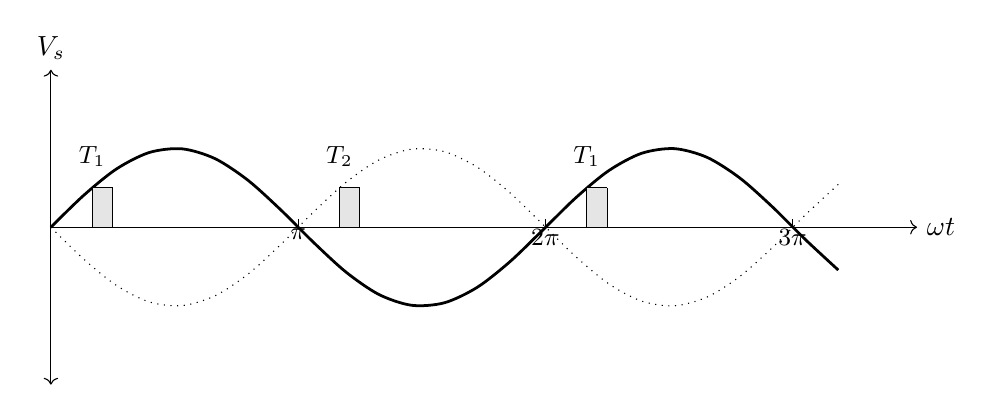
\begin{tikzpicture}[scale=1]
    \draw[->] (0,0) -- (11,0) node[right] {$\omega t$};
    \draw[<->] (0,-2) -- (0,2) node[above] {$V_s$};
    \draw[domain=0:10, smooth, variable=\x, black,line width=1pt] plot ({\x},{sin(deg(\x))});
    \draw[dotted,domain=0:10, smooth, variable=\x, black] plot ({\x},{-sin(deg(\x))});
    \foreach \x/\xtext in {3.14/\pi,6.28/2\pi,9.42/3\pi} {
        \draw (\x cm,0) -- (\x cm,0.1) node[below] {\small$\xtext$};
    }

\fill[gray!20] (0.5233,0) -- (0.5233,0.5) -- (0.785,0.5) -- (0.785,0) -- cycle;
    \fill[gray!20] (3.6633,0) -- (3.6633,0.5) -- (3.925,0.5) -- (3.925,0) -- cycle;
    \fill[gray!20] (6.8033,0) -- (6.8033,0.5) -- (7.065,0.5) -- (7.065,0) -- cycle;

    \draw (0.5233,0) -- (0.5233,0.5);
    \draw (0.5233,0.5) -- (0.785,0.5);
    \draw (0.785,0.5) -- (0.785,0);

    \draw (3.6633,0) -- (3.6633,0.5);
    \draw (3.6633,0.5) -- (3.925,0.5);
    \draw (3.925,0.5) -- (3.925,0);

    \draw (6.8033,0) -- (6.8033,0.5);
    \draw (6.8033,0.5) -- (7.065,0.5);
    \draw (7.065,0.5) -- (7.065,0);


     \node at (0.5233,0.9) {\small$T_1$};
     \node at (3.6633,0.9) {\small$T_2$};
     \node at (6.8033,0.9) {\small$T_1$};
\end{tikzpicture}
\end{figure}
\begin{figure}[!h]
    \centering
    \begin{tikzpicture}[scale=1]
    \draw[->] (0,0) -- (11,0) node[right] {$\omega t$};
    \draw[<->] (0,-2) -- (0,2) node[above] {$V_o$};
    \draw[domain=0.5233:3.14, smooth, variable=\x, black,line width=1pt] plot ({\x},{sin(deg(\x))});
    \draw[domain=3.6633:6.28, smooth, variable=\x, black,line width=1pt] plot ({\x},{-sin(deg(\x))});
    \draw[domain=6.8033:9.42, smooth, variable=\x, black,line width=1pt] plot ({\x},{sin(deg(\x))});

    \foreach \x/\xtext in {0.5233/\alpha, 3.14/\pi,4/\pi + \alpha ,6.28/2\pi,7.2/2\pi + \alpha,9.42/3\pi}{
        \draw (\x cm,0) -- (\x cm,0) node[below] {\small $\xtext$};
    }

     \draw [line width=1pt](0,0)--(0.5233,0);
    \draw [line width=1pt](0.5233,0) -- (0.5233,0.5);
    \draw[line width=1pt](3.14,0)-- (3.6633,0);
    \draw[line width=1pt] (3.6633,0) -- (3.6633,0.5);
    \draw [line width=1pt](6.28,0)--(6.8033,0);
    \draw [line width=1pt](6.8033,0) -- (6.8033,0.5);

    \node at (0.25,0.6){\small$T_2$};
    \node at (0.25,0.2){\small$D_2$};
     \node at (3.4,0.6){\small$T_1$};
    \node at (3.4,0.2){\small$D_1$};
    \node at (6.4,0.6){\small$T_2$};
    \node at (6.4,0.2){\small$D_2$};

    \node at (1.57,0.4){\small $T_1D_2$};
    \node at (4.71,0.4){\small $T_2D_1$};
    
\end{tikzpicture}
\end{figure}
\begin{figure}[!h]
    \centering
    \begin{tikzpicture}[scale=1]
    \draw[->] (0,0) -- (11,0) node[right] {$\omega t$};
    \draw[<->] (0,-2) -- (0,2) node[above] {$i_{T_1}$};
   
    \foreach \x/\xtext in {0.5233/\alpha,4/\pi + \alpha,7.2/2\pi + \alpha,10/3\pi + \alpha}{
        \draw (\x cm,0) -- (\x cm,0) node[below] {\small $\xtext$};
    }
     \draw [line width=1pt](0,0)--(0.5233,0);
    \draw [line width=1pt](0.5233,0) -- (0.5233,1);
    \draw[line width=1pt](0.5233,1)-- (3.6633,1);
    \draw[line width=1pt] (3.6633,1) -- (3.6633,0);
    \draw[line width=1pt] (3.6633,0) -- (6.8033,0);
    \draw [line width=1pt](6.8033,0)--(6.8033,1);
    \draw [line width=1pt](6.8033,1) -- (9.948,1);
     \draw [line width=1pt] (9.948,1) -- (9.948,0);

     \draw[dotted,domain=0:10, smooth, variable=\x, black] plot ({\x},{1});
     \node at (0.4,1.2) {\small $I_{DC}$};
\end{tikzpicture}
\end{figure}
\begin{figure}[!h]
    \centering
    \begin{tikzpicture}[scale=1]
    \draw[->] (0,0) -- (11,0) node[right] {$\omega t$};
    \draw[<->] (0,-2) -- (0,2) node[above] {$i_{s}$};
   

    \draw [line width=1pt](0.5233,0) -- (0.5233,1);
    \draw[line width=1pt](0.5233,1)-- (3.14,1);
    \draw[line width=1pt](3.14,1)-- (3.14,0);
    \draw[line width=1pt] (3.14,0) -- (3.6633,0);
    \draw[line width=1pt] (3.6633,0) -- (3.6633,-1);
    \draw[line width=1pt] (3.6633,-1) -- (6.28,-1);
    \draw[line width=1pt]  (6.28,-1) -- (6.28,0);
    \draw[line width=1pt] (6.28,0) -- (6.8033,0);
    \draw [line width=1pt](6.8033,0)--(6.8033,1);
    \draw [line width=1pt](6.8033,1) -- (9.42,1);
     \draw [line width=1pt] (9.42,1) -- (9.42,0);
     \draw [line width=1pt] (9.42,0) -- (9.948,0);

     \draw[dotted,domain=0:10, smooth, variable=\x, black] plot ({\x},{1});
     \node at (0.4,1.2) {\small $I_{DC}$};
    
\end{tikzpicture}
\end{figure}

From \tabref{tab:inputs.EE.59.2022}:
\begin{align}
   (I_{s_1})_{peak} &= \frac{4I_{dc}}{\pi}\cos{\left(\frac{\alpha}{2}\right)}\\
    &= \frac{4 \times 15 }{\pi}\times \cos{\frac{45 \degree}{2}}\\
    &=17.64 A 
\end{align}

%\end{document}

\pagebreak
\item Consider a system with transfer-function $G\brak{s}=\frac{2}{s+1}$. A unit-step function $\mu\brak{t}$ is applied to the system, which results in an output y\brak{t}. 

If $e\brak{t}=y\brak{t}-\mu\brak{t}$ then $ \lim_{t\to\infty} e(t)$ is\rule{1.5cm}{0.15mm}.
\solution
\iffalse
\let\negmedspace\undefined
\let\negthickspace\undefined
\documentclass[journal,12pt,twocolumn]{IEEEtran}
\usepackage{cite}
\usepackage{amsmath,amssymb,amsfonts,amsthm}
\usepackage{algorithmic}
\usepackage{graphicx}
\usepackage{textcomp}
\usepackage{xcolor}
\usepackage{txfonts}
\usepackage{listings}
\usepackage{enumitem}
\usepackage{mathtools}
\usepackage{gensymb}
\usepackage{comment}
\usepackage[breaklinks=true]{hyperref}
\usepackage{tkz-euclide} 
\usepackage{listings}
\usepackage{gvv}                                        
\def\inputGnumericTable{}                                 
\usepackage[latin1]{inputenc}                                
\usepackage{color}                                            
\usepackage{array}                                            
\usepackage{longtable}                                       
\usepackage{calc}                                             
\usepackage{multirow}                                         
\usepackage{hhline}                                           
\usepackage{ifthen}                                           
\usepackage{lscape}
\newtheorem{theorem}{Theorem}[section]
\newtheorem{problem}{Problem}
\newtheorem{proposition}{Proposition}[section]
\newtheorem{lemma}{Lemma}[section]
\newtheorem{corollary}[theorem]{Corollary}
\newtheorem{example}{Example}[section]
\newtheorem{definition}[problem]{Definition}
\newcommand{\BEQA}{\begin{eqnarray}}
\newcommand{\EEQA}{\end{eqnarray}}
\newcommand{\define}{\stackrel{\triangle}{=}}
\theoremstyle{remark}
\usepackage{circuitikz}
\newtheorem{rem}{Remark}
\begin{document}
\parindent 0px

\bibliographystyle{IEEEtran}
\vspace{3cm}

\title{Assignment\\[1ex]GATE-IN-46}
\author{EE23BTECH11034 - Prabhat Kukunuri$^{}$% <-this % stops a space
}
\maketitle
\newpage
\bigskip

\renewcommand{\thefigure}{\theenumi}
\renewcommand{\thetable}{\theenumi}
\section{Question}
Consider a system with transfer-function $G\brak{s}=\frac{2}{s+1}$. A unit-step function $\mu\brak{t}$ is applied to the system, which results in an output y\brak{t}. 

If $e\brak{t}=y\brak{t}-\mu\brak{t}$ then $ \lim_{t\to\infty} e(t)$ is\rule{1.5cm}{0.15mm}.

\solution
\fi
\begin{table}[h]
    \centering
    \begin{tabular}{|p{1cm}|p{3.00cm}|p{3.50cm}|}
    \hline
    Symbol&Value&Description\\ \hline
    $$G\brak{s}$$&$$\frac{2}{s+1}$$&$$\text{Transfer function}$$\\\hline
    $$e\brak{t}$$&$$y\brak{t}-\mu\brak{t}$$&$$\text{Function of y\brak{t} and $\mu\brak{t}$}$$\\\hline
    $$Y\brak{s}$$&$$G\brak{s}\times U\brak{s}$$&Convolution in $t$ domain is multiplication in $s$ domain.\\\hline
    $$\mu\brak{t}$$&$$\begin{cases}
    0&\text{if t$<$0}\\
    1&\text{if t$>$0}
    \end{cases}$$&$$\text{Unit step function}$$\\\hline
    \end{tabular}
    \caption{Variable description}
    \label{tab:GATE.2021.IN.46.1}
\end{table}\\
Applying Laplace transform on $\mu\brak{t}$
\begin{align}
    &\mu\brak{t}\system{L}U\brak{s}\\
    &U\brak{s}=\frac{1}{s}\\
    &Y\brak{s}=\brak{\frac{2}{s+1}}\brak{\frac{1}{s}}\\
    &Y\brak{s}=\frac{2}{s}-\frac{2}{s+1}
\end{align}
The inverse Laplace transform of $\frac{a}{s+b}$ is $ae^{-bt}\mu\brak{t}$
\begin{align}
    &y\brak{t}=2\mu\brak{t}-2e^{-t}\mu\brak{t}\\
    &e\brak{t}=\mu\brak{t}\brak{1-2e^{-t}}\\
    &\lim_{t\to\infty}e\brak{t}=\lim_{t\to\infty}\mu\brak{t}\brak{1-2e^{-t}}\\
    &\lim_{t\to\infty}e\brak{t}=1
\end{align}
%\end{document}

\pagebreak
\item  Solution of differential equation $y'' + y'+ 0.25y = 0$ with initial values $y(0) = 3$ and $y'(0) = -3.5$ is
\begin{enumerate}
    \item[(A)] $ y = (3-2x)e^{0.5x} $
    \item[(B)] $ y = (3-2x)e^{-0.25x}$
    \item[(C)] $ y = (3-2x)e^{-0.5x}$
    \item[(D)] $ y = (2-3x)e^{-0.5x}$
\end{enumerate} 
\hfill(GATE AG 2021) \\
\solution
\iffalse
\let\negmedspace\undefined
\let\negthickspace\undefined
\documentclass[journal,12pt,twocolumn]{IEEEtran}
\usepackage{cite}
\usepackage{amsmath,amssymb,amsfonts,amsthm}
\usepackage{algorithmic}
\usepackage{graphicx}
\usepackage{textcomp}
\usepackage{xcolor}
\usepackage{txfonts}
\usepackage{listings}
\usepackage{enumitem}
\usepackage{mathtools}
\usepackage{gensymb}
\usepackage{comment}
\usepackage[breaklinks=true]{hyperref}
\usepackage{tkz-euclide} 
\usepackage{listings}
\usepackage{gvv}                                        
\def\inputGnumericTable{}                                 
\usepackage[latin1]{inputenc}                                
\usepackage{color}                                            
\usepackage{array}                                            
\usepackage{longtable}                                       
\usepackage{calc}                                             
\usepackage{multirow}                                         
\usepackage{hhline}                                           
\usepackage{ifthen}                                           
\usepackage{lscape}
\usepackage{amsmath}
\usepackage{caption}

\newtheorem{theorem}{Theorem}[section]
\newtheorem{problem}{Problem}
\newtheorem{proposition}{Proposition}[section]
\newtheorem{lemma}{Lemma}[section]
\newtheorem{corollary}[theorem]{Corollary}
\newtheorem{example}{Example}[section]
\newtheorem{definition}[problem]{Definition}
\newcommand{\BEQA}{\begin{eqnarray}}
\newcommand{\EEQA}{\end{eqnarray}}
\newcommand{\define}{\stackrel{\triangle}{=}}
\theoremstyle{remark}
\newtheorem{rem}{Remark}
\begin{document}

\bibliographystyle{IEEEtran}
\vspace{3cm}

\title{GATE: AG-26 2021}
\author{EE23BTECH11038 - Rohith Madhani$^{*}$% <-this % stops a space
}
\maketitle
\newpage
\bigskip
\renewcommand{\thefigure}{\theenumi}
\renewcommand{\thetable}{\theenumi}

\textbf{Question :} Solution of differential equation $y'' + y'+ 0.25y = 0$ with initial values $y(0) = 3$ and $y'(0) = -3.5$ is
\begin{enumerate}
    \item[(A)] $ y = (3-2x)e^{0.5x} $
    \item[(B)] $ y = (3-2x)e^{-0.25x}$
    \item[(C)] $ y = (3-2x)e^{-0.5x}$
    \item[(D)] $ y = (2-3x)e^{-0.5x}$
\end{enumerate} 
\hfill(GATE AG 2021) \\
\solution
\fi

\begin{table}[!h] 
    \centering
    \begin{table}[!ht] 
\centering
\setlength{\extrarowheight}{8pt}
\begin{tabular}{|l|l|l|}
    \hline
    \textbf{Parameter} & \textbf{Description} & \textbf{Values}\\
    \hline
     m & load of system &  \\
    \hline
     k & stiffness of system &  \\
    \hline
     $\omega_n$ & Natural frequency & $\sqrt{\frac{k}{m}}$ \\
    \hline
    $\zeta$ & Damping ratio & $\frac{c}{2m\omega_n}$ \\
    \hline
     y\brak{t} & Output of system & \\
    \hline
     x\brak{t} & Input to the system & \\
    \hline
     c & Damping coefficient & \\
    \hline
    T\brak{s} & Transfer function of system & $\frac{Y\brak{s}}{R\brak{s}}$\\
    \hline
  \end{tabular}
  \vspace{4mm}
 \caption{Parameter Table}
 \label{tab:table0_ee_22_39}
\end{table}

    \caption{Given parameters}
    \label{table:gate21ag26}
\end{table}
By applying laplace transform to the differential equation,
\begin{align}
    y''+y'+0.25y &\Large\xleftrightarrow{\mathcal{L}} s^2Y(s)-sy(0)-y'(0)+sY(s)-y(0)+0.25Y(s)
\end{align}

\begin{align}
    Y(s)(s^2 + s + 0.25) &= 3s - 0.5 \\
    \implies Y(s) &= \frac{3s-0.5}{s^2 + s + 0.25} \\
    &= \frac{3}{s+0.5} - \frac{2}{(s+0.5)^2};Re(s) > -0.5 \label{parfrac}
\end{align}

As we know,
\begin{align}
    \frac{b}{(s+a)^n} &\Large\xleftrightarrow{\mathcal{L}^{-1}}\frac{b}{(n-1)!} t^{n-1} e^{-at} u(t)
\end{align}

By taking inverse laplace of \eqref{parfrac}, we get
\begin{align}
    y(t) &= \frac{3}{0!}e^{-0.5t}u(t)-\frac{2}{1!}te^{-0.5t}u(t) \\
    \implies y(t) &= \sbrak{(3-2x)e^{-0.5t}}u(t)
\end{align}
Hence the correct answer is option (C)
\newpage

\begin{figure}[t]
    \centering
    \includegraphics[width=\columnwidth]{2021/AG/26/figs/fig1.png}
    \caption{$y(t) = \sbrak{(3-2t)e^{-0.5t}}u(t)$}
    \label{fig:gate21ag26}
\end{figure}

%\end{document}

\pagebreak
\item Consider the following first order partial differential equation, also known as the transport equation
\begin{align*}
\frac{\partial y\brak{x,t}}{\partial t}+5\frac{\partial y\brak{x,t}}{\partial x}&=0
\end{align*}
with initial conditions given by $y(x, 0) = \sin x,-\infty < x < \infty$. The value of $y(x, t)$ at $x = \pi$ and $t=\frac{\pi}{6}$ is  \rule{1cm}{0.15mm}.
\begin{enumerate}[label=(\Alph*)]
\item 1
\item 2
\item 0
\item 0.5
\end{enumerate}
\hfill(GATE 2021 BM Q28)\\
\solution
\input{2021/BM/28/28.tex}
\pagebreak
\item In the circuit, switch 'S' is in the closed position for a very long time. If the switch is opened at time $t=0$, then $i_L\brak{t}$ in amperes, for $t\geq0$ is
\begin{figure}[h]
    \renewcommand\thefigure{1}
    \centering
    \begin{circuitikz}[american]
    \draw (0,0) to (1,0) to (1,-2) to [R=$4\Omega$] (3,-2) to [V=$30V$,invert] (5,-2) to (5,0) to  [R=$1\Omega$] (7,0) to [L=$0.5H$] (7,-4) to (0,-4) to [V=$10V$,invert] (0,0);
    % Draw the open switch
    \draw (1,0) to[ospst] (5,0);
    % Add a label for the open switch
    \node at (3,0.8) {\scriptsize{Open at $t=0$}};
    % Draw the arrow and label for current
    \draw [->] (6.6,-1.4) -- (6.6,-2.7);
    \node at (6.4,-1.9) {$i_{L}$};
    \end{circuitikz}
    \caption{Circuit in $T$ domain}
    \label{fig:EE_21_29_1}
\end{figure}
\\
\hfill(GATE 2021 EE 29)\\
\solution
\iffalse
\let\negmedspace\undefined
\let\negthickspace\undefined
\documentclass[journal,12pt,twocolumn]{IEEEtran}
\usepackage{cite}
\usepackage{circuitikz}
\usepackage{amsmath,amssymb,amsfonts,amsthm}
\usepackage{algorithmic}
\usepackage{graphicx}
\usepackage{textcomp}
\usepackage{xcolor}
\usepackage{txfonts}
\usepackage{listings}
\usepackage{enumitem}
\usepackage{mathtools}
\usepackage{gensymb}
\usepackage{comment}
\usepackage[breaklinks=true]{hyperref}
\usepackage{tkz-euclide} 
\usepackage{listings}
\usepackage{gvv}                                        
\def\inputGnumericTable{}                                 
\usepackage[latin1]{inputenc}                                
\usepackage{color}                                            
\newtheorem{theorem}{Theorem}[section]
\usepackage{array}                                            
\usepackage{longtable}                                       
\usepackage{calc}                                             
\usepackage{multirow}                                         
\usepackage{hhline}                                           
\usepackage{ifthen}                                           
\usepackage{lscape}
\newtheorem{problem}{Problem}
\newtheorem{proposition}{Proposition}[section]
\newtheorem{lemma}{Lemma}[section]
\newtheorem{corollary}[theorem]{Corollary}
\newtheorem{example}{Example}[section]
\newtheorem{definition}[problem]{Definition}
\newcommand{\BEQA}{\begin{eqnarray}}
\newcommand{\EEQA}{\end{eqnarray}}
\newcommand{\define}{\stackrel{\triangle}{=}}
\theoremstyle{remark}
\newtheorem{rem}{Remark}
\begin{document}
\bibliographystyle{IEEEtran}
\vspace{3cm}
\title{GATE 21 EE/29}
\author{EE23BTECH11040 - Manoj Kumar Ambatipudi$^{*}$% <-this % stops a space
}
\maketitle
\newpage
\bigskip
\renewcommand{\thefigure}{\theenumi}
\renewcommand{\thetable}{\theenumi}
\textbf{QUESTION:}
In the circuit, switch 'S' is in the closed position for a very long time. If the switch is opened at time $t=0$, then $i_L\brak{t}$ in amperes, for $t\geq0$ is
\begin{figure}[h]
    \renewcommand\thefigure{1}
    \centering
    \begin{circuitikz}[american]
    \draw (0,0) to (1,0) to (1,-2) to [R=$4\Omega$] (3,-2) to [V=$30V$,invert] (5,-2) to (5,0) to  [R=$1\Omega$] (7,0) to [L=$0.5H$] (7,-4) to (0,-4) to [V=$10V$,invert] (0,0);
    % Draw the open switch
    \draw (1,0) to[ospst] (5,0);
    % Add a label for the open switch
    \node at (3,0.8) {\scriptsize{Open at $t=0$}};
    % Draw the arrow and label for current
    \draw [->] (6.6,-1.4) -- (6.6,-2.7);
    \node at (6.4,-1.9) {$i_{L}$};
    \end{circuitikz}
    \caption{Circuit in $T$ domain}
    \label{fig:EE_21_29_1}
\end{figure}
\\
\hfill(GATE 2021 EE 29)
\textbf{Solution:}
\fi
\begin{table}[h]
\renewcommand\thetable{1}
    \centering
    \begin{tabular}{|c|c|c|}
    \hline
         Variables&Description&value  \\\hline
            $i_L\brak{0}$   &    Initial current in Inductor & 10A\\\hline
            L     & Inductance of Inductor & 0.5H\\\hline
    \end{tabular}
    \caption{Caption}
    \label{tab:EE_21_29_1}
\end{table}

Circuit in $S$ domain is
\begin{figure}[h]
\renewcommand\thefigure{2}
    \centering
    \begin{circuitikz}[american]
    \draw (0,0) to (0.9,0) to (0.9,-2) to [generic=$4\Omega$] (2.9,-2) to [V=$\frac{30}{s}V$,invert](4.9,-2) to (4.9,0) to  [generic=$1\Omega$](6.9,0) to [generic=$0.5s$](6.9,-2) to [V=$Li_L\brak{0}$,invert](6.9,-4) to (0,-4) to [V=$\frac{10}{s}V$,invert](0,0);
    \draw (0.9,0) to[ospst] (4.9,0);
    % Add a label for the open switch
    \node at (3,0.8) {\scriptsize{Open at $t=0$}};
    \end{circuitikz}
    \caption{Circuit in $S$ domain}
    \label{fig:EE_21_29_2}
\end{figure}
\\
From \figref{fig:EE_21_29_1}, $i_L\brak{0}$ can be found using steady state analysis. Writing $KVL$ , we get
\begin{align}
    10-i_L\brak{0} &= 0\\
    i_L\brak{0} &= 10\label{eq:EE_21_29_1}
\end{align}
Writing $KVL$ for \figref{fig:EE_21_29_2},
\begin{align}
    \frac{10}{s} - I_L\brak{s}\brak{4+1+0.5s} + \frac{30}{s} + Li_L\brak{0} &= 0\\
    \implies I_L\brak{s} &= \frac{sLi_L\brak{0}+40}{5s + 0.5s^2} 
\end{align}
From \tabref{tab:EE_21_29_1}, 
\begin{align}
    I_L\brak{s} &= \frac{2.5s+40}{5s + 0.5s^2}\\
    I_L\brak{s} &= \frac{10s+80}{10s + s^2}\\
                &= \frac{8}{s} + \frac{2}{s+10}
\end{align}
Taking Inverse Laplace, 
\begin{align}
    i_L\brak{t} &= \brak{8+2e^{-10t}}u\brak{t}
\end{align}
\begin{figure}[h]
\renewcommand\thefigure{3}
    \centering
    \includegraphics[width=1.0\columnwidth]{2021/EE/29/figs/fig_3.jpg}
    \caption{Plot of $i_L\brak{t}$ taken from Python3}
    \label{fig:EE_21_29_3}
\end{figure}

\pagebreak
\end{enumerate}
